\section{Auswertung}
\label{sec:Auswertung}

Im nun Folgenden werden die aufgenommenen Messdaten der verschiedenen Scans ausgewertet. 


\subsection{Detektorscan}
\label{sec:Detektorscan}

Zu Beginn wird anhand des Detektorscans die Halbwertsbreite und die maximale Intensität bestimmt.
Hierfür wird eine Gaußfunktion der Form
\begin{equation}
    I(\theta)= A \cdot \exp \left(-\frac{(\theta-\mu)^2}{2 \sigma^2}\right)+b
\end{equation}
an die Messdaten gefittet.
Die daraus resultierenden Parameter ergeben sich zu 
\begin{align*}
    a & = \qty{4.34(64)e4}{} \, , \\
    b & = \qty{9.48(1.87)e3}{} \, , \\
    \sigma & = \qty{3.614(0.054)e-2}{} \, \text{und} \\
    \mu & = \qty{1.07(0.51)e-3}{\degree} \, .
\end{align*}
Die Halbwertbreite und die maximale Intensität ergiben sich zu
\begin{align*}
    I_max &= \qty{4.89e5}{} \\
    \text(FWHM) &= \qty{8.63e-2}{\degree}
\end{align*}
Die Regression ist in \autoref{fig:Detektorscan} zu sehen.
\begin{figure}
    \centering
    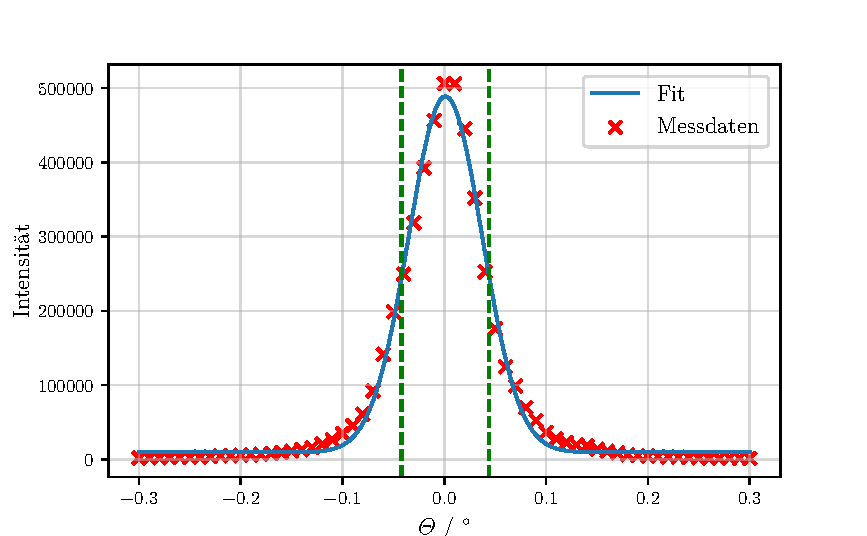
\includegraphics[width = 0.5 \linewidth]{build/Detektorscan.pdf}
    \caption{Fit der Gaußfunktion an die Messdaten.}
    \label{fig:Detektorscan}
\end{figure}

\subsection{Z-Scan}

\begin{figure}
    \centering
    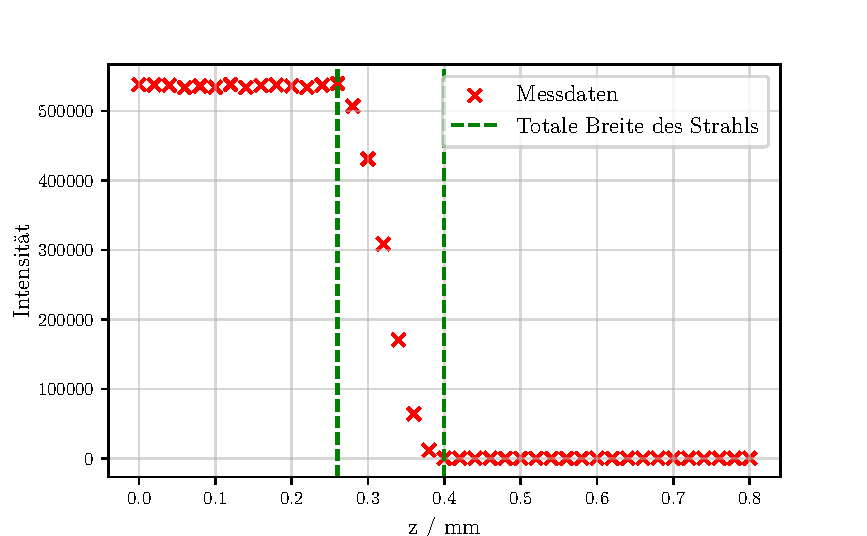
\includegraphics[width = 0.5 \linewidth]{build/z_scan.pdf}
    \caption{Messdaten des Z-Scans und Analyse zur Strahlbreite.}
    \label{fig:z_scan}
\end{figure}

Mithilfe des Z-Scans kann die Strahlbreite des Röntgenstrahls abgeschätzt werden.
Die Messdaten zum Versuch und die Analyse sind in \autoref{fig:z_scan} zu finden.
Die Strahlbreite ergibt sich zur $d_0 = 0.14 \unit{\milli\meter}$.

\subsection{X-Scan}

\begin{figure}
    \centering
    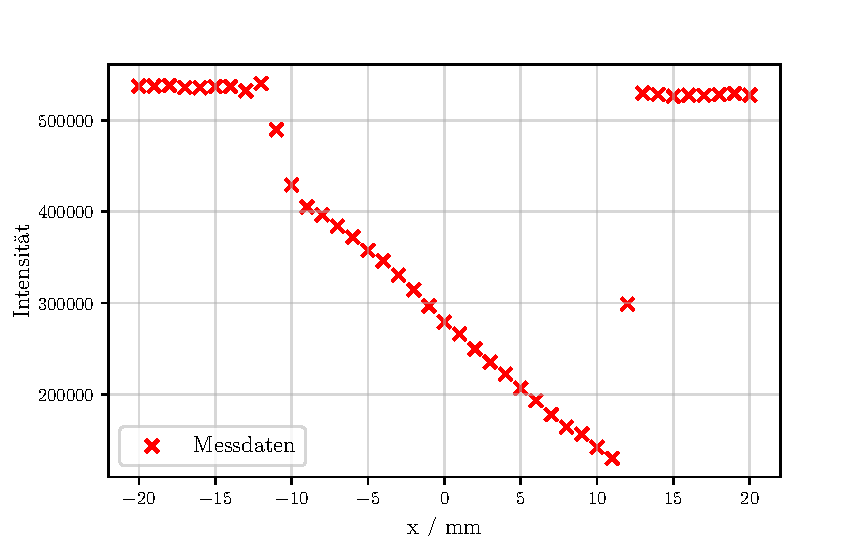
\includegraphics[width = 0.5 \linewidth]{build/x_scan.pdf}
    \caption{Messdaten des X-Scans.}
    \label{fig:x_scan}
\end{figure}

Des weiteren wird der X-Scan zur Bestimmung der Position der Probe durchgeführt.
Die Messdaten finden sich in \autoref{fig:x_scan} wieder.
Im Anschluss der Messung wurde eine beliebige Position innerhalb des Intervalls der Probe gewählt.

\subsection{Rockingscan}

\begin{figure}
    \centering
    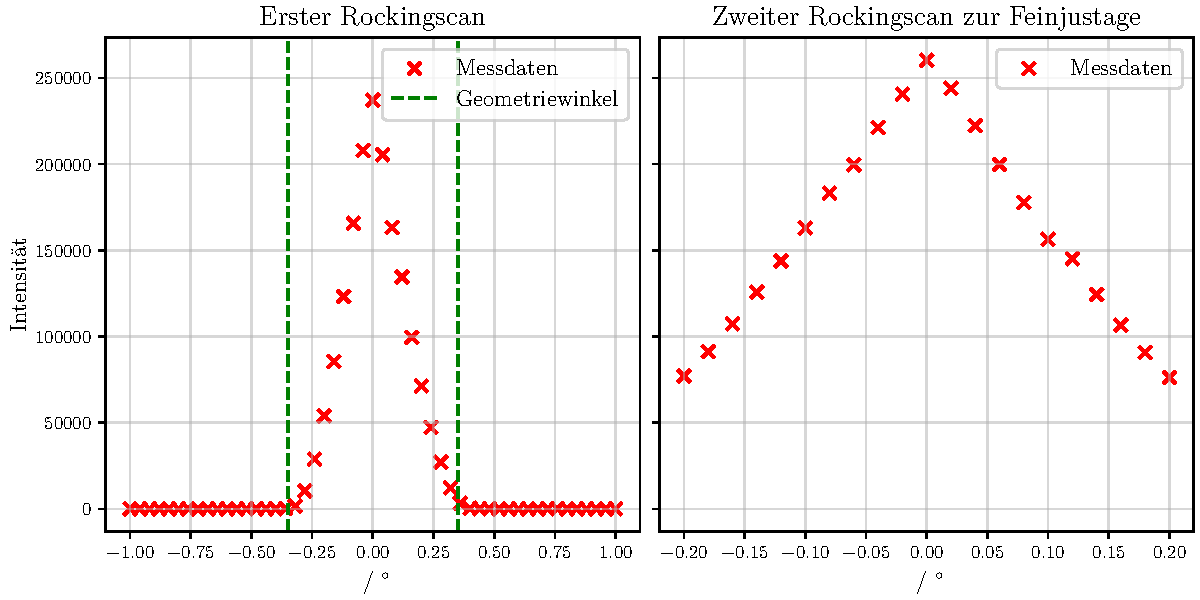
\includegraphics[width = 0.5 \linewidth]{build/rockingscan.pdf}
    \caption{Rockingscan zur Analyse des Auflagewinkels der Probe.}
    \label{fig:rockingscan}
\end{figure}

Wie in \autoref{sec:Durchführung} beschrieben, wird jetzt ein Rockingscan durchgeführt, um die Verkippung der Probe zu korrigieren.
Diese Analyse wird auch genutzt um den Geometriewinkel abzuschätzen.
Diese Abschätzung und die Messdaten sind in \autoref{fig:rockingscan} zu sehen.
Der Geometriewinkel ergibt sich dabei zu $\theta_\text{Geom} \approx 0.35 °$.
Der theoretische Geometriewinkel ergibt sich durch 
\begin{equation*}
    \theta_\text{Geom, Theo} = arcsin\left(\frac{d_0}{D}\right) = 0.401 \unit\degree \, .
\end{equation*}
Dabei ist $D = 20 \unit{\milli\meter}$ und beschreibt die Ausmaße der Probe.

\subsection{Messung}

\begin{figure}
    \centering
    \includegraphics[width = 0.5 \linewidth]{build/messreihe1.pdf}
    \caption{Reflektivität aufgetragen gegen den Winkel.}
    \label{fig:messreihe1}
\end{figure}

Nachdem die Apperatur nach \autoref{sec:Durchführung} justiert wurde, wird nun die tatsächliche Messung durchgeführt.
Die Messdaten sind in \autoref{fig:messreihe1} zu sehen.
Hier ist die normale, \enquote{direkte} Messung abzüglich der diffusen Messung aufgetragen.
Es sei angemerkt, dass hier bereits die Intensität in die Reflektivität umgewandelt wurde.
Diese berechnet sich durch $R = \frac{I}{ 5 \cdot I_\text{max}}$.
Die Minima der Kiessig Oszillationen sind ebenfalls eingezeichet.
Berechnet wurden sie durch die Python Bibliothek \textit{SciPy}, beziehungsweise durch \textit{scipy.signal.argrelextrema}.
Dabei wurden nur Minima führender Ordnung angegeben, da in einem größeren Winkelbereich die Messung zu ungenau wird.
Nun müssen die Abstände dieser Minima berechnet werden und gemittelt werden.
Diese Rechnung ergibt
\begin{equation*}
    \delta \omega = (0.059 \pm 0.022) \unit\degree \, .
\end{equation*}
Mit diesen Größen kann nun die Schichtdicke $d$ bestimmt werden.
Dafür wird die allgemein bekannte Wellenlänge der $K_\alpha$ Linie von $\lambda = 1, 541 \cdot 10^-10$ in \autoref{eq:schichtdicke} eingesetzt.
Die Rechnung ergibt
\begin{equation*}
    d = (1.3 \pm 0.49) \cdot 10^-9 \, .
\end{equation*}